%!TEX output_directory = build
%!TEX aux_directory = build


\documentclass[12pt]{article}
\usepackage{lingmacros}
\usepackage{tree-dvips}
\usepackage{amsmath}               
\usepackage{amsthm}
\usepackage{float}
\usepackage{multirow}
\usepackage{array}
\usepackage{subfigure}
\usepackage{afterpage}
\usepackage{amsmath,amssymb}            
\usepackage{rotating}  
\usepackage{fancyhdr}  
\usepackage{cancel}
\usepackage{tabularx}
\usepackage{multicol}
\usepackage{hyperref}
\usepackage{filecontents}
\usepackage{listings}
\usepackage{nomencl}
\usepackage{hyperref}
\usepackage{textcomp}
\usepackage{mathrsfs}
\usepackage{epigraph}
\usepackage[T1]{fontenc}
\usepackage[utf8]{inputenc}
\usepackage{xcolor}
%\usepackage[italian]{babel}
%\usepackage[latin1]{inputenc}
\usepackage[english]{babel}
\usepackage[nodisplayskipstretch]{setspace}
\setstretch{1.2}

\begin{document}

\newcommand{\fix}[1]{\textcolor{red}{FIX: #1} }   

\section*{Stability}

Once the NMPC problem has been formulated and the feasibility of the problem has been analized as in Equation \ref{feasibility} guaranteeing the fulfillment of hard  constraints, its stability has to be investigated. A proof of a terminal constraint-free approach for a nonlinear MPC is presented in \cite{alamir2018stability}, anyway our approach, parameterizing the control action, lead to some difficulties in assessing the stability with standard approaches. \\
We will consider now the tracking problem as a zero-reference tracking problem. In order to do that we will consider:
\begin{equation}\label{change_var}
    e_k=x_k-{x_d}_k
\end{equation}
and so, substituting \ref{change_var} in the state equation \ref{state_eq_param}, we can define:
\begin{equation} \label{NLsystem}
	\hat{f}^+(e_{k|i},p_k,{{x_d}_{k|i}},{{x_d}_{k|i+1}},t_i) = \tilde{f}^+(e_{k|i}-{x_d}_k,p_k,t_i)
\end{equation}
then the discrete error state equation becomes:
\begin{equation}\label{sys_eq_con_e}
    e_{k|i+1}=\hat{f}^+(e_{k|i},p_k,{{x_d}_{k|i}},{{x_d}_{k|i+1}},t_i)=\hat{f}^+(e_{k|i},p_k,t_i)
\end{equation}
Note that, for simplicity of notation, the system equation in \ref{sys_eq_con_e} has been expressed as a function of the state error ${e_{k|i}}$ and the parameters $p_k$ only, given that the desired states are known.\\
In this way the problem is moved to track a zero error reference and becomes: 
\begin{equation} \label{ourproblem_stab}
\begin{split}
		& min_{{p}_k}\ J({e}_{k|0},{p}_k) =\sum_{i=1}^{N}\left(\frac{i}{N}\right)^b\hat{h}(e_{k|i},{p}_{k}) \\
		\textnormal{s.t.}\qquad
		&\ \ \ \ e_{k|i+1}=\hat{f}^+(e_{k|i},p_k,t_i) \\
		&\ \ \ \ e_{k|i} \in \mathbb{E}\ \forall\ i=1,\dots,\ N  \\
		&\ \ \ \ {p}_k\   \in \mathbb{P}\ \\
	\end{split}	
\end{equation}
where $\mathbb{E} = \lbrace {e}\in \mathbb{R}^n\ \textnormal{s.t.}\ {e}_{min}\leq e\leq e_{max} \rbrace$ is the feasible region of the state error and $\hat{h}$ is the stage cost function in \ref{costfunctionh} considering the change of variables in Equation \ref{change_var}. 

Now, requiring that the point $e=0$ is a stable equilibrium point for the closed loop system means to asses if J is a Lyapunov function, i.e. to assess if: 
\begin{equation}
	J({e}_{k+1|0},{p^*}_{k+1}) \leq J({e}_{k|0},{p^*}_k)
	\label{lyap_stab}
\end{equation}
Usually the most used approaches to verify this relies on a terminal constaint for the problem (i.e. $e_N=0$) or requiring the existance of a terminal set.
Anyway, the novelty of our approach lies in the absence of the terminal constraint and on the parameterization of the control action. Because of this last one, the extension of what done in \cite{alamir2018stability} is not straitforward and requires more general considerations. 

What we will do is firstly to require that the parameterization is such that allows to be translatable. In other words, given the optimal solution at time instant $k$ defined as $p_k^*=\left[ p_{k_1}^*,\ p_{k_2}^*,  \dots,\ p_{k_{N_p}}^* \right]^T$ that corresponds to $  \textbf{u}_k^*=[\ u_{k|0}^*,\ u_{k|1}^*,\  \dots,\  u_{k|{N-1}}^*\ ]$, we will require that it is possible to obtain the parameter $\tilde{p}_{k+1}$ such that the correspondent control input is $  \tilde{\textbf{u}}_{k+1}=[\ u_{k|1}^*,\ u_{k|2}^*,\  \dots,\  u_{k|{N-1}}^*,\ u_{k|N}^* \ ]$. A clear grapical rapresentation of this can be seen in Figure \ref{param_translatability}. \fix{sarebbe da metter a posto questa immagine sotto}
\begin{figure}[h!]
	\centering
	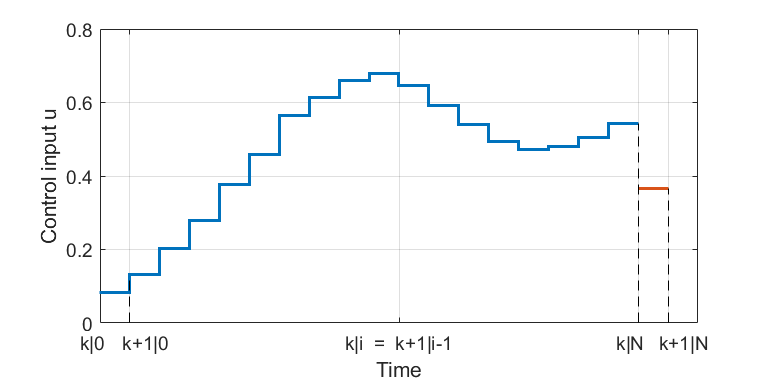
\includegraphics[scale=0.6]{IMMAGINI/trans_u.png}
	\caption{Translatability of the $F$ function}
	\label{param_translatability}
\end{figure}

To understand the stability of the closed loop system we will consider the cost function generated from this last $\tilde{p}_{k+1}$:

\begin{equation}
	J({e}_{k+1|0},\tilde{p}_{k+1})=\sum_{i=1}^{N}\left(\frac{i}{N}\right)^b\hat{h}(e_{k+1|i},\tilde{p}_{k+1})
\end{equation}

and for the definition of $\tilde{p}_{k+1}$ we can relate this last cost to the optimal cost at the previous step: 


\begin{equation}
\begin{split}
	J({e}_{k+1|0},\tilde{p}_{k+1})&=\sum_{i=1}^{N}\left(\frac{i}{N}\right)^b\hat{h}(e_{k+1|i},\tilde{p}_{k+1}) \\
	&=\sum_{i=2}^{N}\left(\frac{i}{N}\right)^b\hat{h}(e_{k|i},p^*_{k}) + \hat{h}(\hat{f}^+(e_{k|N},p^*_k,t_N)) \\
\end{split}
\label{interm_stab}
\end{equation}

and noting that the first term of the last equation is part of the optimal cost function at instant $k$:

\begin{equation}
	\sum_{i=2}^{N}\left(\frac{i}{N}\right)^b\hat{h}(e_{k|i},p^*_{k})=J({e}_{k|0},p^*_k) -\left( \frac{1}{N} \right)^b\hat{h}(e_{k|1},p^*_{k})
\end{equation}

equation \ref{interm_stab} can then be rewritten as:

\begin{equation}
\begin{split}
	J({e}_{k+1|0},\tilde{p}_{k+1})=J({e}_{k|0},p^*_k) -\left( \frac{1}{N} \right)^b\hat{h}(e_{k|1},p^*_{k}) + \hat{h}(\hat{f}^+(e_{k|N},p^*_k,t_N)) \\
\end{split}
\end{equation}

and rearranging the terms:

\begin{equation}
\begin{split}
	\underbrace{J({e}_{k+1|0},\tilde{p}_{k+1})-J({e}_{k|0},p^*_k)}_{D}= \hat{h}(\hat{f}^+(e_{k|N},p^*_k,t_N)) -\left( \frac{1}{N} \right)^b\hat{h}(e_{k|1},p^*_{k}) \\
\end{split}
\end{equation}

The $D$ term is of of high interest because if we are able to demonstrate that $D$ is negative or equal to zero, the stability of the system is definitively assessed. The reason lies in the fact that, saying that $D\leq0$, for the definition of optimality of the solution implies also that: $J({e}_{k+1|0},{p^*}_{k+1}) - J({e}_{k|0},{p^*}_k) \leq 0$, i.e. the \ref{lyap_stab} holds. Therefore, we will analyze if the equation $D\leq0$ admit a solution for any $k$, this means to show that the equation: 
\begin{equation}
\begin{split}
	\hat{h}(\hat{f}^+(e_{k|N},p^*_k,t_N))-\left( \frac{1}{N} \right)^b\hat{h}(e_{k|1},p^*_{k}) \leq 0 \\
\end{split}
\end{equation}
is always true for any $k$. \\

Rearanging the terms we can rewrite: 

\begin{equation}
\begin{split}
	\left( \frac{1}{N} \right)^b \geq \frac{\hat{h}(\hat{f}^+(e_{k|N},p^*_k,t_N))}{\hat{h}(e_{k|1},p^*_{k})}=\frac{C_1}{C_2} \\
\end{split}
\end{equation}

This last equation contains the main problem in assessing the stability: depending on the value of the ratio $\frac{C_1}{C_2}$ the value of the exponent $b$ that ensure the stability changes.\\
What can be said is that theoretically always exists a value of $b$ for which the point $e=0$ is a stable equilibrium point for the closed loop system. But more in general we want the value of $b$ to be fixed and positive and this analisys cannot guarantee the value of the ratio $\frac{C_1}{C_2}$ to be bounded and $\leq 1$, for example we can also have $C_2=0$ that implies that we need $b=\infty$ which is not practically possible.\\
For those reasons, assessing the stability of the system that lies in showing that 
\begin{equation}
	J({e}_{k+1|0},\tilde{p}_{k+1})-J({e}_{k|0},p^*_k) \leq 0
\end{equation}
means that we are requiring the $\tilde{p}_{k+1}$ to decrease the cost function. This requirement, as shown in \cite{alamir_boh}, can be verified by looking at solving time and solver capabilities.
\fix{Quest'ultima ref è il paper di alamir che ti avevo mandato} \\
\fix{Se la tesi è dire quello che abbiamo imparato da questa cosa e spiegare onestamente mi sembra che questo sia quello che ho capito io di questo problema. Ho detto qualcosa anche nelle conclusioni sul fatto che la stabilità rimane un problema aperto}.

\end{document}